
\subsection{Adding a New Account}
\label{sec:add-account}

The Add New Account screen enables users to add a new account by specifying the account's name, currency used and starting balance. The user can also specify whether or not to use this account as the default account to use for everyday transactions.

\subsubsection{Application Screenshots}
\begin{figure}[h]
 
\begin{subfigure}{0.5\textwidth}
  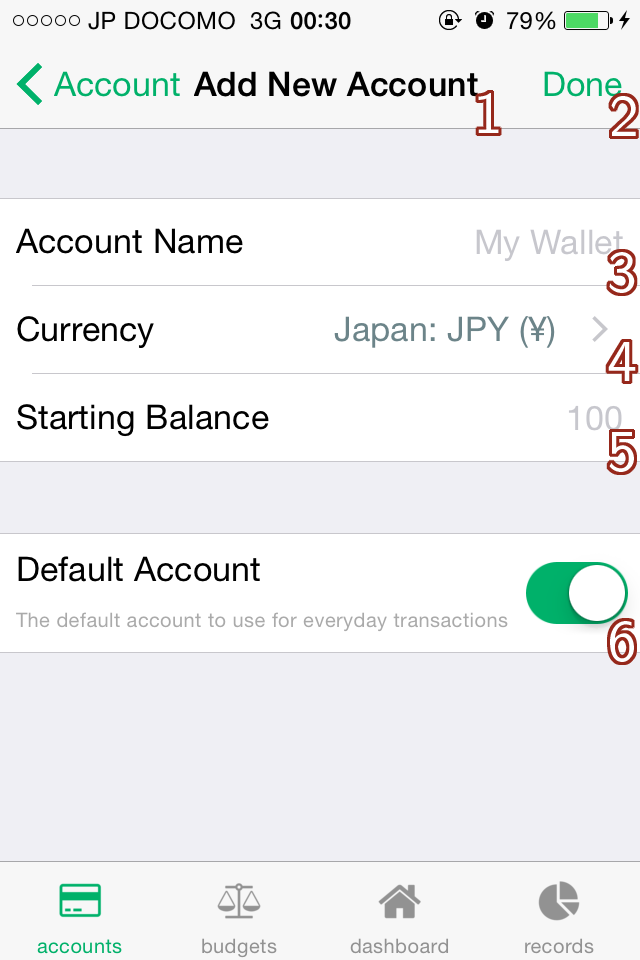
\includegraphics[scale=0.35]{ACC-0001-1} 
  \caption{Add New Account Screen}
  \label{fig:sub-account-1}
\end{subfigure}
\begin{subfigure}{0.5\textwidth}
  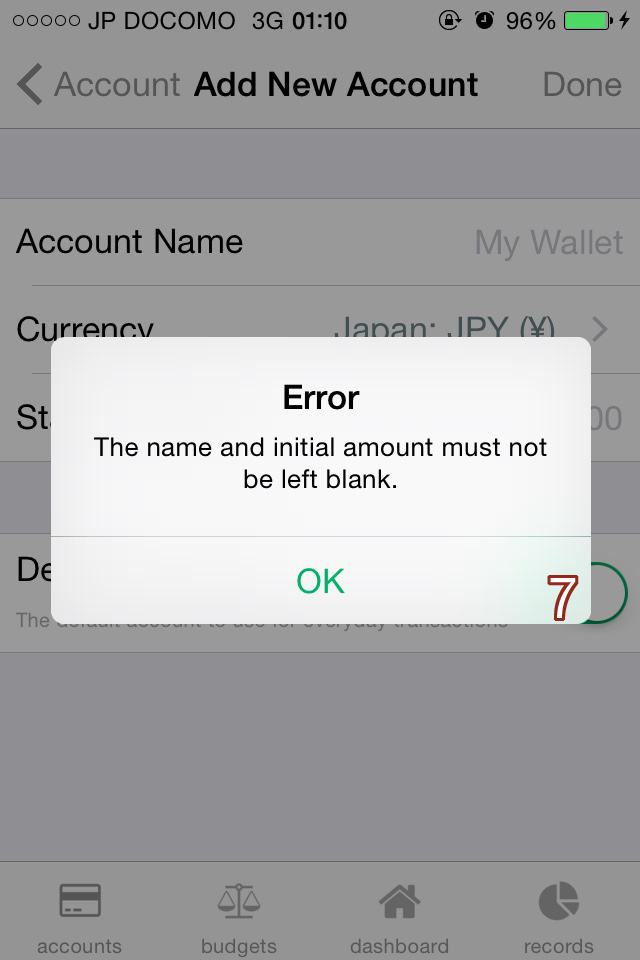
\includegraphics[scale=0.35]{ACC-0001-4}
  \caption{Error Scenario}
  \label{fig:sub-account-2}
\end{subfigure}
\caption{Add New Account Screenshots}
\end{figure}

\screentable{
	\header{Screen Component}
    	{Type}
        {Description}
    \row{1. Screen Title}
    	{Label Title}
        {Localization Key: MENULABEL\_ADD\_ACCOUNT}
    \row{2. Done Button}
    	{Button}
        {
        When tapped, the app performs form validation and saves all the account information -- the account name, currency, starting balance, and whether or not to use the account as default -- into the database. \doublenewline
        For more details on the form validation, please see Section 4.1.2. \doublenewline
        Localization Key: BUTTON\_DONE
        } 
    \row{3. Account Name Cell}
    	{Table Cell}
        {This table cell consists of two UI elements: A label and a textfield. \doublenewline
        
        Tap anywhere in the cell and the textfield will be placed in focus, bringing up a QWERTY keyboard. Tap anywhere outside the cell to dismiss the keyboard. \doublenewline
        
        The textfield has a character limit of 25 characters.\doublenewline
        
        Localization Keys: LABEL\_NAME, TEXTFIELD\_NAME\_PLACEHOLDER} 
    \row{4. Currency Cell}
    	{Table Cell}
        {This table cell consists of two UI Label elements. \doublenewline
        
        When this table cell is tapped, the cell will be briefly filled with a light green background, then fade out as the screen transitions to the Currency Selection screen. The default currency depends on the user's device locale.\doublenewline 
        
        Localization Key: LABEL\_CURRENCY} 
}

\screentable{
	\header{Screen Component}
    	{Type}
        {Description}
    \row{5. Starting Balance Cell}
    	{Table Cell}
        {This table cell consists of two UI elements: A label and a textfield. \doublenewline
        
        Tap anywhere in the cell and the textfield will be placed in focus, bringing up a keyboard that is numeric with a decimal point.  Tap anywhere outside the cell to dismiss the keyboard. \doublenewline
        
        The textfield has a character limit of 15 characters.\doublenewline
         
        Localization Keys: LABEL\_STARTING\_BALANCE, TEXTFIELD\_STARTING\_BALANCE\_ PLACEHOLDER} 
    \row{6. Default Account Cell}
    	{Table Cell}
        {This table cell consists of three UI elements: two labels and a switch. The switch is turned off by default.\doublenewline
        
        Tap anywhere in the cell and the switch will be toggled. There can only be one default account at any time. \doublenewline
        
        Localization Keys: LABEL\_IS\_DEFAULT\_ACCOUNT, LABEL\_IS\_DEFAULT\_ACCOUNT\_ DESCRIPTION} 
    \row{7. Error Alert}
    	{Alert Controller}
        {This alert controller has two labels. \doublenewline
        
        The alert is displayed when either the account name or the initial amount has not been filled, and the user taps \"Done\".\doublenewline
        
        Localization Keys: ERRORLABEL\_ERROR\_TITLE, ERRORLABEL\_NAME\_CURRENCY\_ NOT\_EMPTY}
}

\subsubsection{Error Scenarios}

\errortable{
	\errorheader{Title}{Description}
    \errorrow{Duplicate Account Name}
    	{This error is triggered when the Done button is pressed and a similar account name already exists in the Core Data. \doublenewline
        
        Localization Key: ERRORLABEL\_ DUPLICATE\_ACCOUNT\_NAME}
    \errorrow{Required Fields Unfilled}
    	{This error is triggered when the Done button is pressed and the account name or the amount has not been filled. \doublenewline
        
        Localization Key: ERRORLABEL\_NAME\_CURRENCY\_ NOT\_EMPTY}
    
    \errorrow{Multiple Decimals}
    	{This check confirms that decimals can only be inputted once. It only exists in textfields that have numeric input. \doublenewline
        
        If a decimal is in the input, and the user keys in another decimal point, the textfield will not respond. There will be no error alert displayed. \doublenewline
        
        If the user pastes text that has two decimal points, then the textfield will not respond as well. Once again, there will be no error alert displayed.
        }
        
    \errorrow{Maximum Length}
    	{This check confirms that the length of the input text is less than or equal to a given number. It is present in all textfields. \doublenewline
        
        Once the maximum length is reached, the user will no longer be able to input any new character. No error alert is displayed.\doublenewline
        
        If the user pastes text that is longer than the maximum length, it will fail to paste and no error alert is displayed.}
}

\subsubsection{Use Cases}
